\documentclass[10pt, letterpaper, oneside]{book}
\usepackage[left=1in, right=1in, bottom=1in, top=1.5in]{geometry}
\usepackage{amsfonts}  %fonts like \mathbb{}
\usepackage{amssymb,amsmath}
\usepackage{graphicx}
%\usepackage{mathrsfs} %for\mathscr
\usepackage[mathscr]{euscript}
\usepackage[colorlinks=true,urlcolor=blue,linkcolor=blue]{hyperref} % navega por el doc
\usepackage{hyperref} %h yperref of equations
\usepackage{amsthm}   %for \theoremstyle, \begin{proof}

% Theorems and definitions
\theoremstyle{theorem} % for put not italic letters
\newtheorem{theorem}{Theorem}%[section]         % Teoremas
\theoremstyle{theorem} % for put not italic letters
\newtheorem{lemma}{Lemma}%[section]         % Lemas
\theoremstyle{definition}
\newtheorem{definition}{Definition}%[section]   % Definiciones
\theoremstyle{remark}
\newtheorem*{remark}{Remark}              % Observaciones
\theoremstyle{definition}
\newtheorem{example}{Example}%[section]         % Ejemplos
\theoremstyle{definition}
\newtheorem{exercise}{Excersice}%[section]      % Ejercicios
\theoremstyle{theorem} 
\newtheorem{proposition}{Proposición}%[section] % Proposición

% Definitions 
\def\Re{\mathbb{R}}
\def\Z{\mathbb{Z}}
\def\Fu{\mathscr{F}}
\def\be{\begin{equation}}
\def\ee{\end{equation}}
\def\bth{\begin{theorem}}
\def\eth{\end{theorem}}
\def\ble{\begin{lemma}}
\def\ele{\end{lemma}}
\def\bde{\begin{definition}}
\def\ede{\end{definition}}
\def\bex{\begin{example}}
\def\eex{\end{example}}
\def\bpr{\begin{proof}}
\def\epr{\end{proof}}
\def\bre{\begin{remark}}
\def\ere{\end{remark}}

\renewcommand{\implies}{\Rightarrow}
\newcommand{\mb}[1]{\mathbf{#1}} % Math bold face

\title{Lectures on General Relativity}
\author{Juan Guarin, Antonio Calixto}
\date{\today}

\begin{document}
%\maketitle
\begin{center}
	\huge
	\textbf{Lectures on General Relativity}
	
	\vspace{5mm}
	Juan Andrés Guarín-Rojas, and\\
	Antonio Calixto Gutiérrez-Piñeres
	
	\vspace{5mm}
	%August 30th, 2023
	\today
\end{center}
\vfill
\begin{figure}[hb]
	\centering
	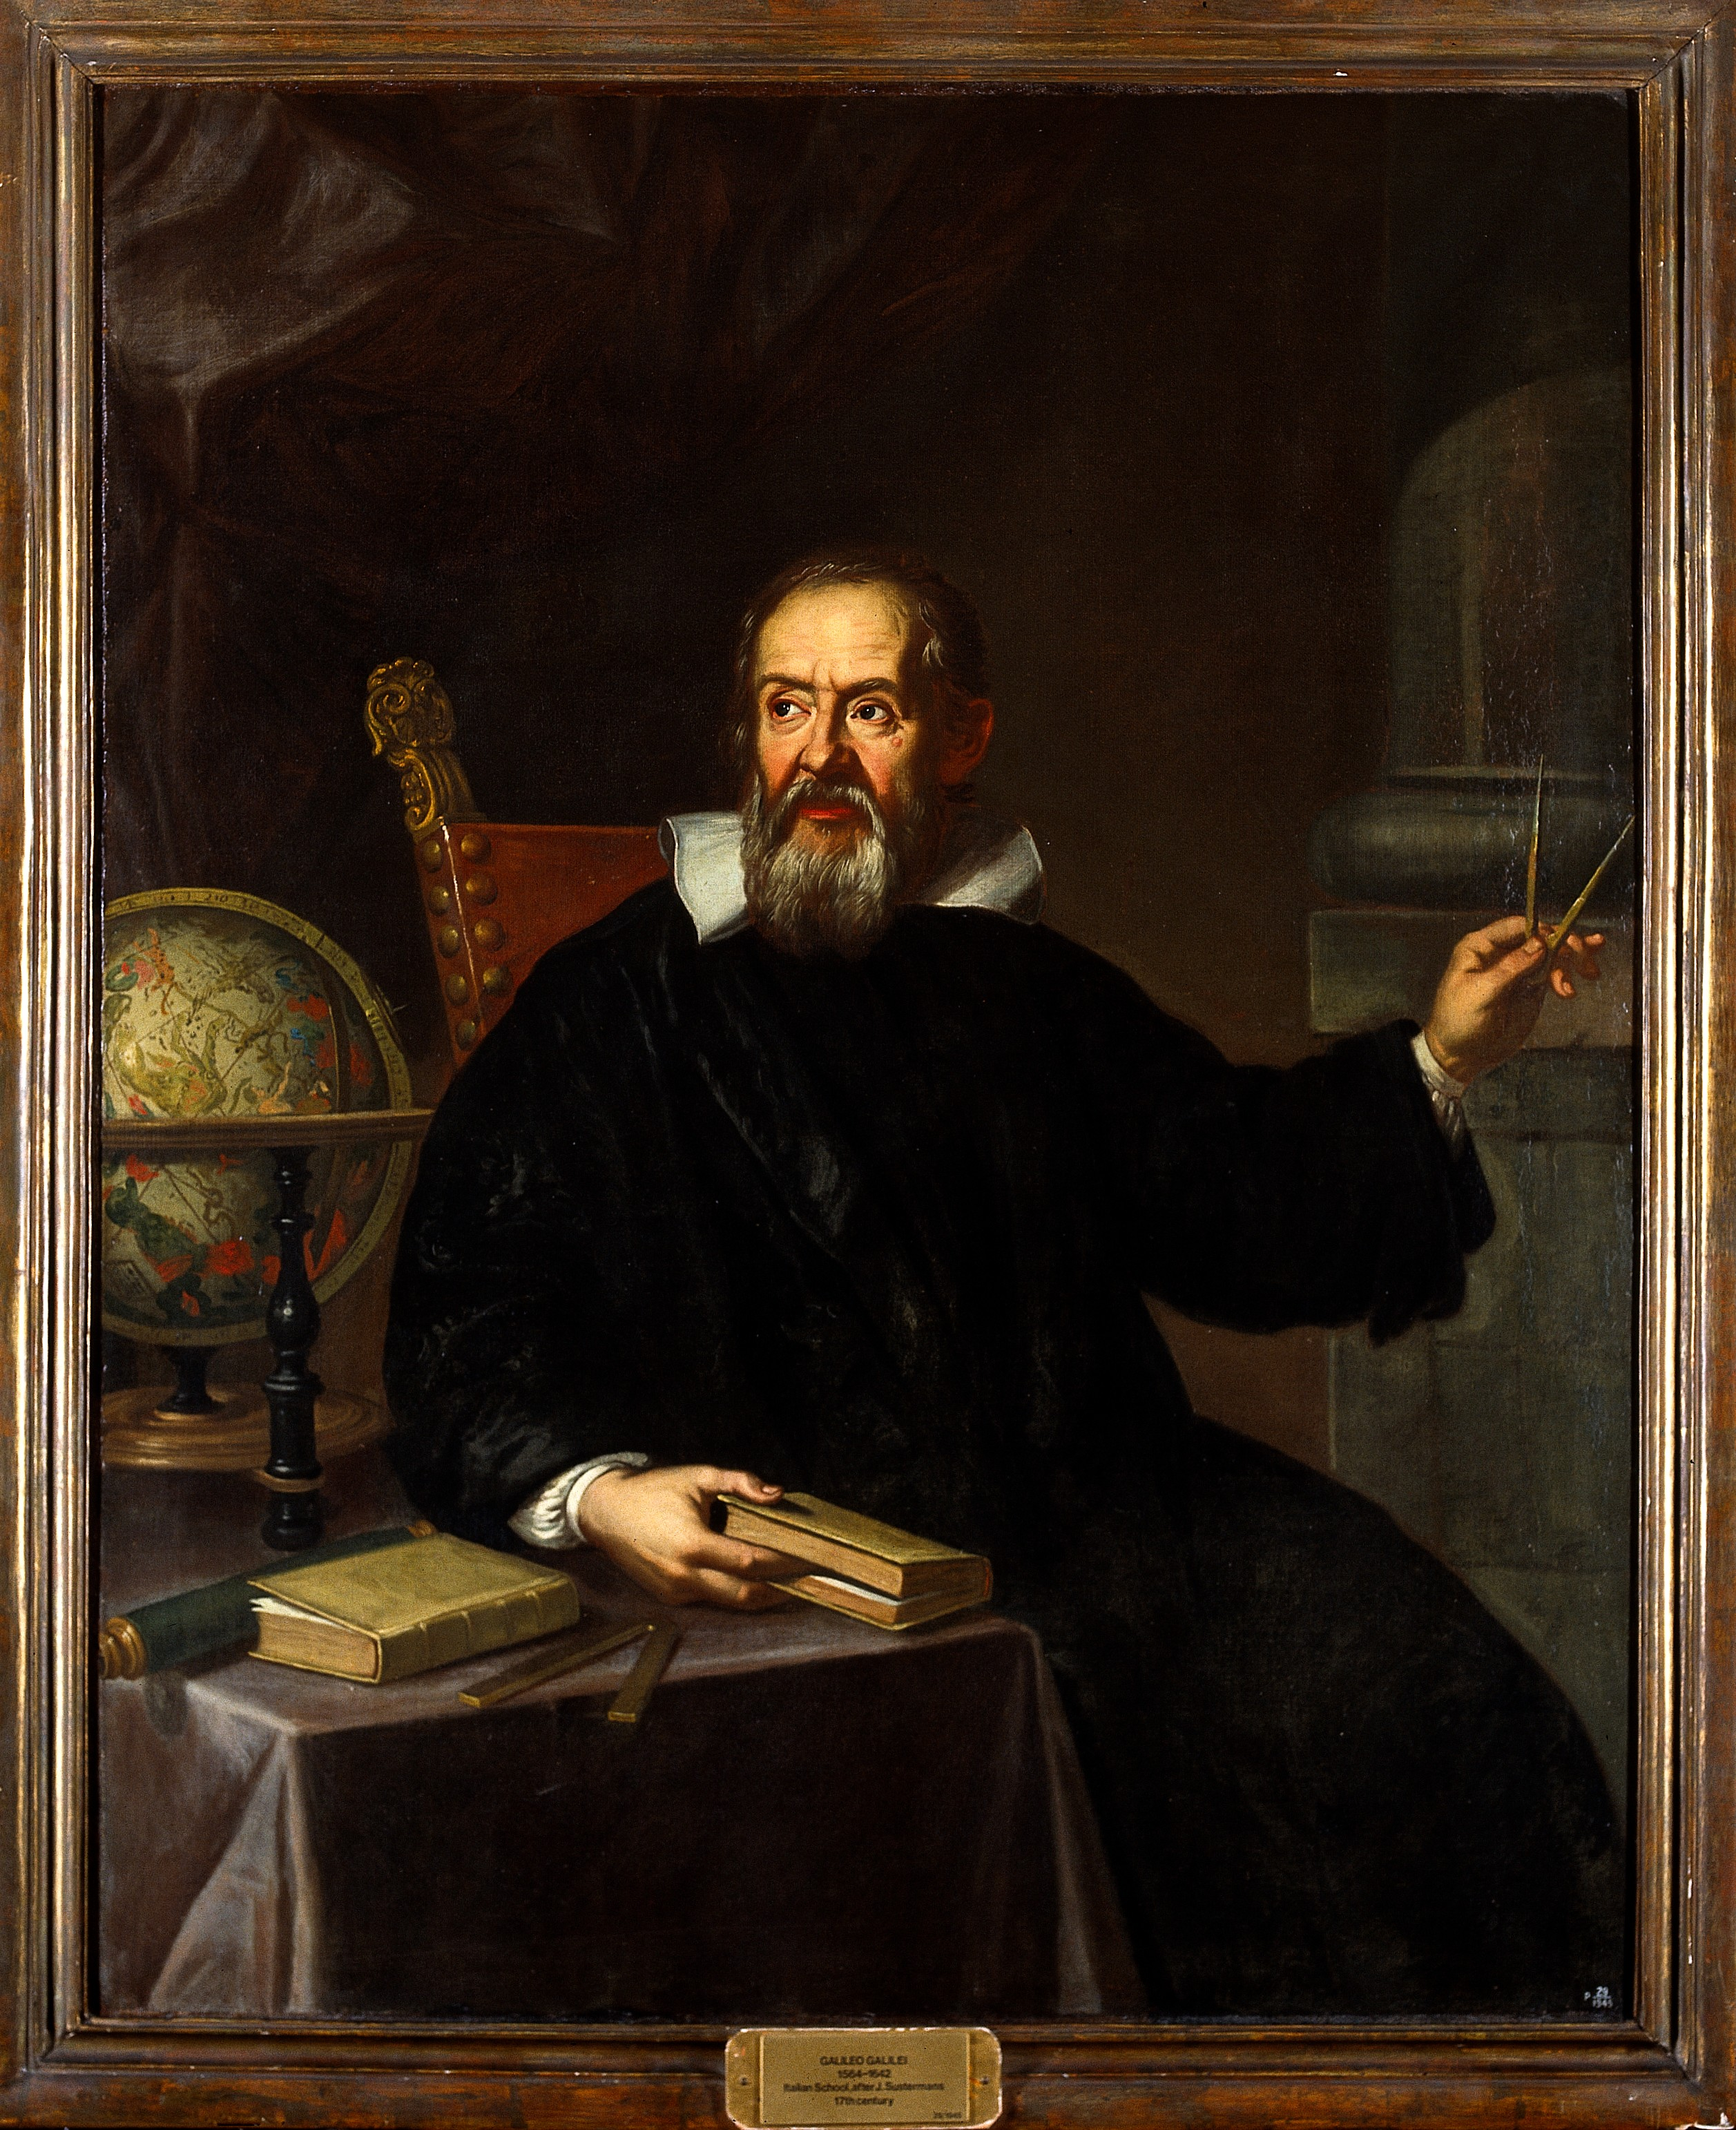
\includegraphics[width=0.7\linewidth]{images/Galileo-Galilei.jpg}
	%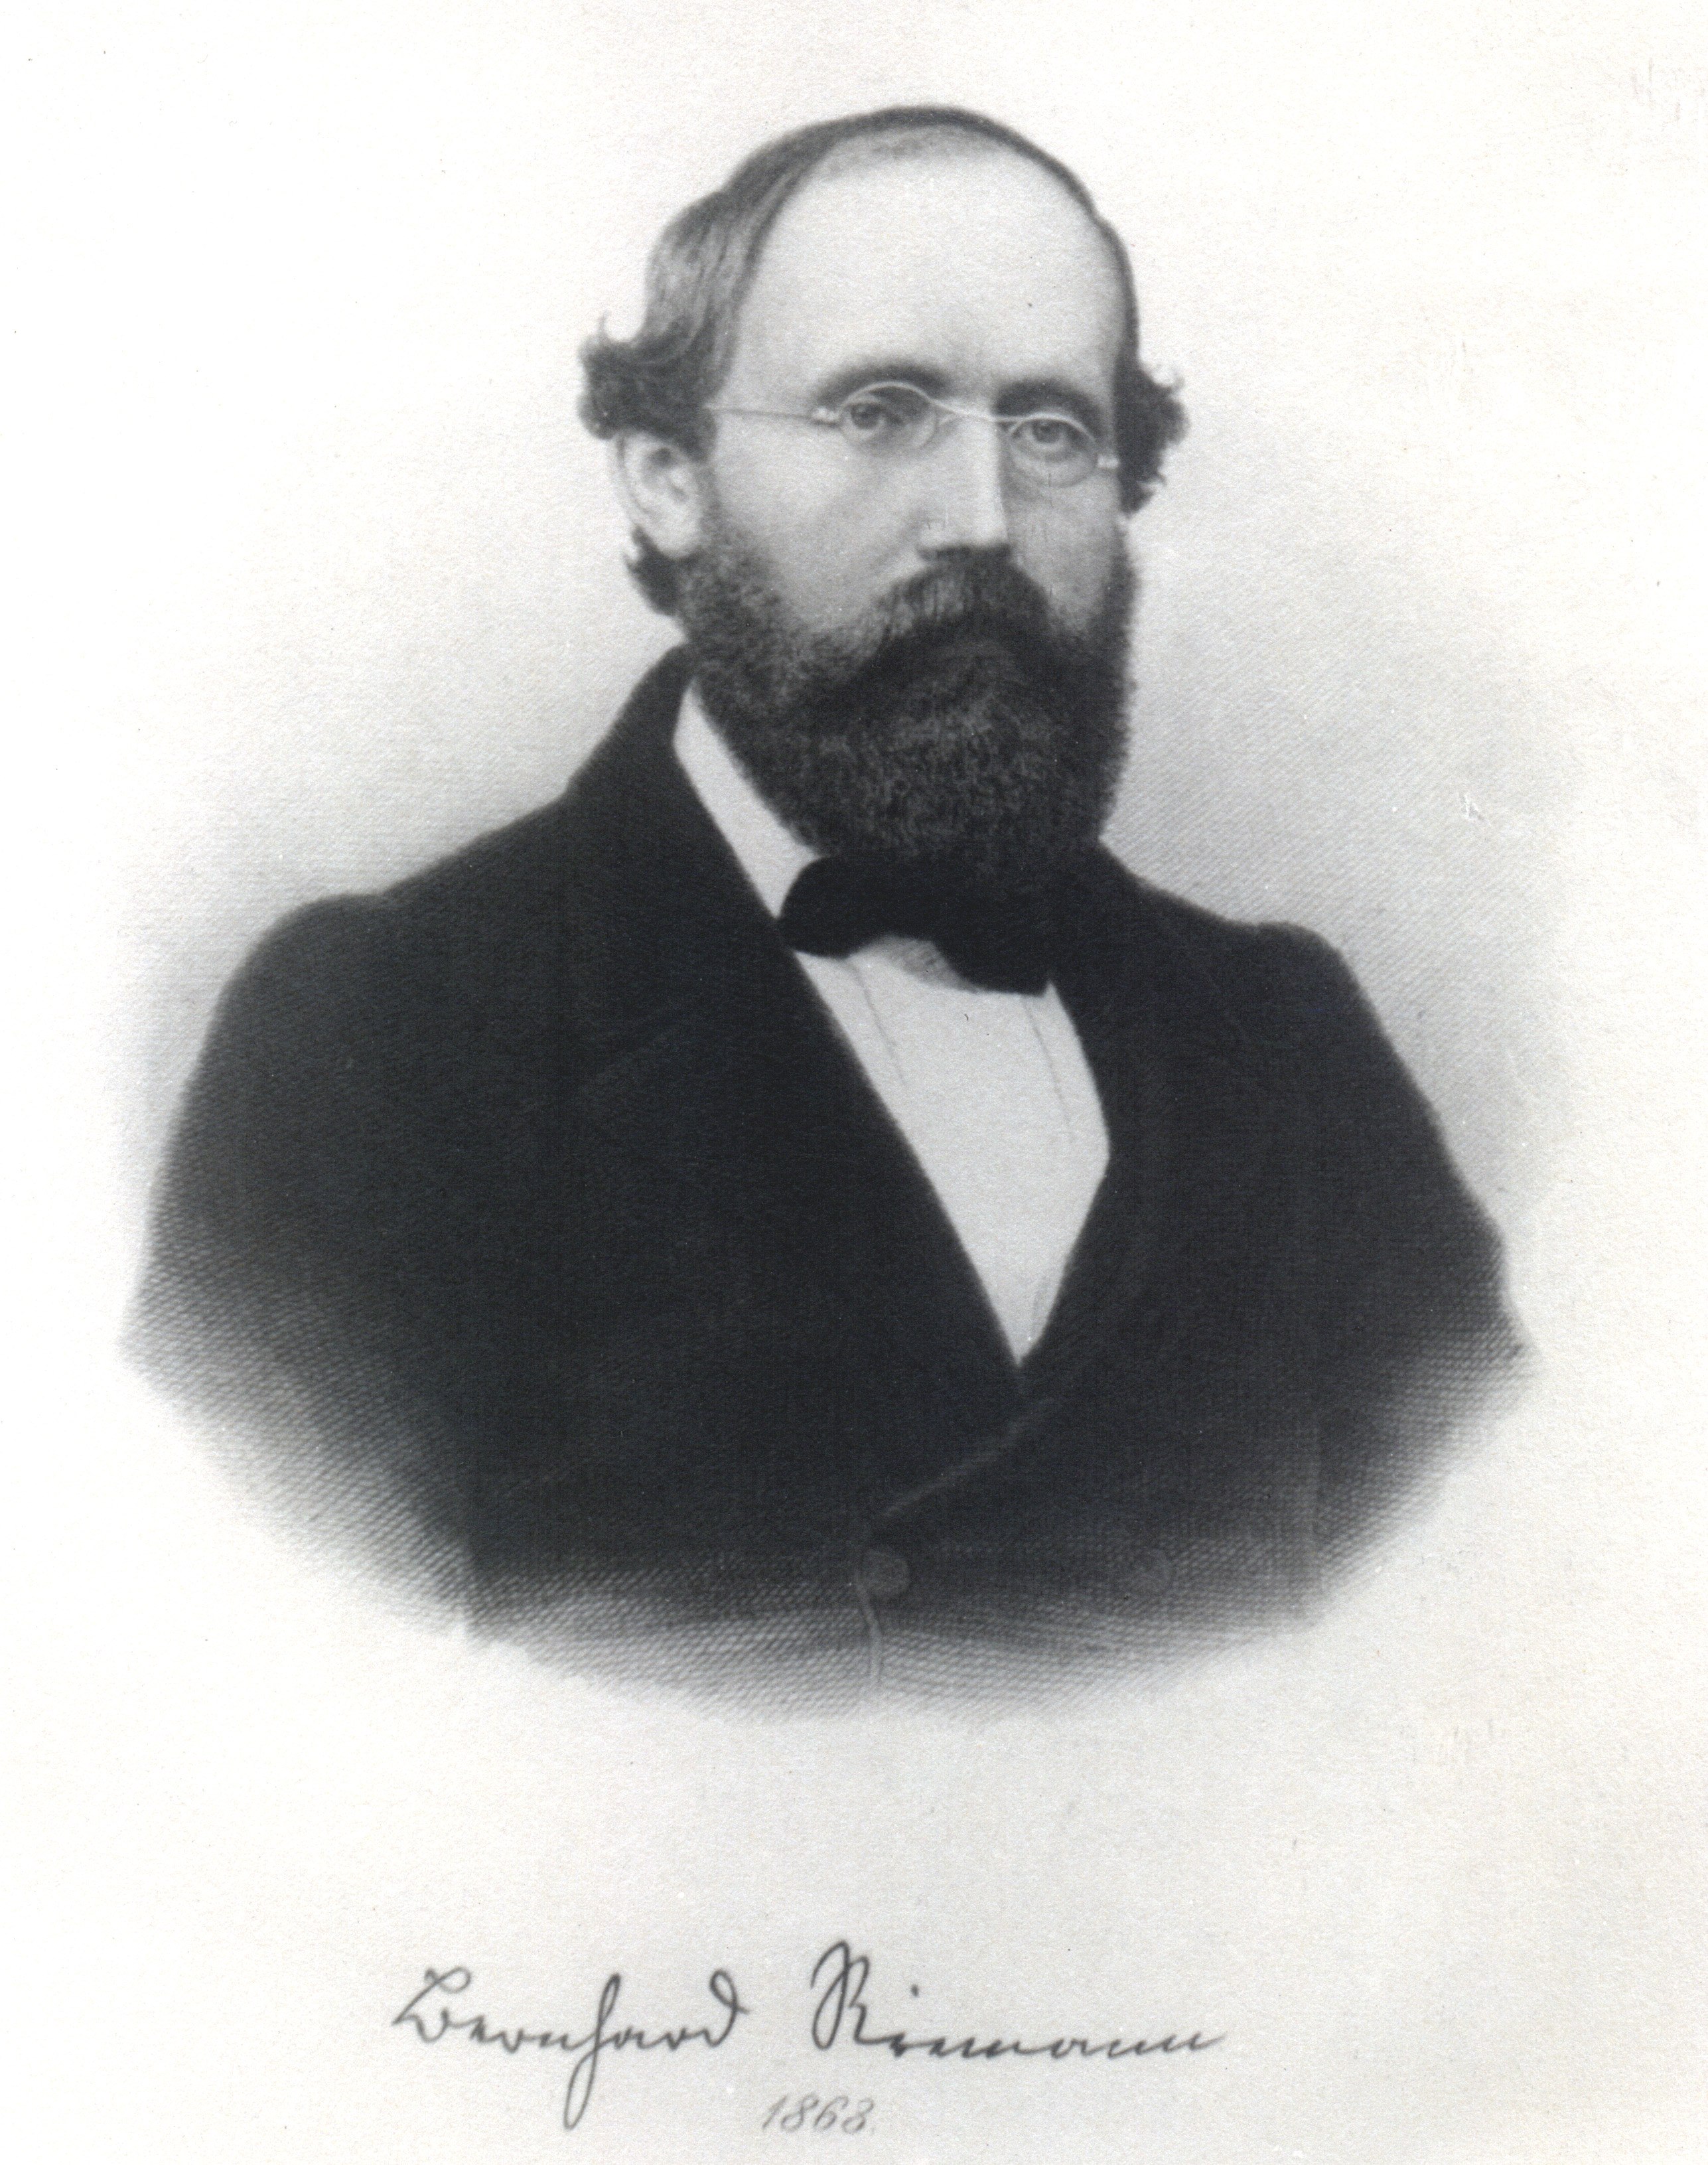
\includegraphics[width=0.7\linewidth]{images/Portrait_of_Bernhard_Riemann.jpg}
\end{figure}
\vfill

\newpage

\textit{Was du ererbt von deinen Vätern hast, Erwirb es, um es zu besitzen}

\rule{\linewidth}{0.4pt}
\begin{flushright}
\textsc{goethe}
\end{flushright}

%\noindent
\begin{figure}[ht]
	\centering
	\includegraphics[width = 0.7\linewidth]{images/Rene_magritte-the_beautiful_realities.jpg}
	\caption{\textit{Les Belles Realités}, René Magritte. ADAGP, Paris, 1984.}
\end{figure}

\tableofcontents

%%%%%%%%%%%%%%%%%%%%%%%%%%%%%%%%%%%%%%%%%%%%%%%%%%%%%%%%%%%%%%%%%%%%%%%%%%%%%%%%%%%%%%%%%%%%%%%%%%%%%%%%%%%%%%%%%%%%%%%%%%%%%%%%%%%%%%%%%%%%%%%%%%%%%%%%%%%%%%%%%%%%%%%%%%%%%%%%%%%%%%%%%%%%%%%%%%%%%%%%%%%%
\chapter{Fundamentals of Classical Mechanics}
\section{Constrains Imposed by the Principle of Relativity}
The Galileo's Principle of Relativity is \cite{arnold}:
\textit{There exist coordinate systems, called intertial, possesing the following properties:}
\begin{itemize}
	\item[\textit{1}] \textit{All the laws of the nature at all moments of time are the same in all inertial coordinate systems.}
	\item[\textit{2}] \textit{All coordinate systems in uniform rectilinear motion with respect to an inertial one are themselves inertial.}
\end{itemize}

The phrase \textit{All the law of nature at all moments of time are the same...} is related to time invariance. The time invariance means that if $\mb{x}={\boldsymbol \varphi}(t)$ is a solution of the Newton equation
\begin{equation}
	\ddot{\mb{x}} = \mb{F}(\dot{\mb{x}},\mathbf{x},t)
\end{equation}
then for any $s\in\Re$, $\mb{x}={\boldsymbol \varphi}(t+s)$ is also a solution. This only means that if we parametrize a movement in a starting point $t_0$ and then in another time translated to the first $t_0+\Delta t$ then the physic law does not change it keeps its form. Nature laws of physics must not change over time, they remain the same now, in the past, and in the future. We can prove that this requirement is only possible if the Newton equation is a homogeneus differential equation:

Let ${\boldsymbol \varphi}$ be a general solution of the ordinary differential equation $\ddot{\mb{x}}=\mb{F}(\dot{\mb{x}},\mb{x},t)$. By Galileo's Principle of Relativity ${\varphi}$ is also a solution by changing $t\mapsto t+s$, then:
\begin{equation}
	\tilde{\boldsymbol \varphi}(t)={\boldsymbol \varphi}(t+s)
\end{equation}
By differentiating both side twice in $t$ we get:
\begin{equation}
	\ddot{\tilde{\boldsymbol \varphi}}(t)=\ddot{\boldsymbol \varphi}(t+s)
\end{equation}
As they both are solutions to the Newton equation then:
\begin{equation}
	\mb{F}\left(\tilde{\boldsymbol \varphi}(t),\dot{\tilde{\boldsymbol \varphi}}(t),t\right) = \mb{F}\left({\boldsymbol \varphi}(t+s),\dot{\boldsymbol \varphi}(t+s),t+s\right)
\end{equation}
By definition of $\tilde{\boldsymbol \varphi}$ we have:
\begin{equation}
	\mb{F}\left({\boldsymbol \varphi}(t+s),\dot{\boldsymbol \varphi}(t+s),t\right) = \mb{F}\left({\boldsymbol \varphi}(t+s),\dot{\boldsymbol \varphi}(t+s),t+s\right)
\end{equation}
The only way that this can be true is that:
\begin{equation}
	\frac{\partial \mb{F}({\boldsymbol \varphi},\dot{\boldsymbol \varphi},t)}{\partial t}=0 \Longleftrightarrow \mb{F}=\mb{F}({\boldsymbol \varphi},\dot{\boldsymbol \varphi})
\end{equation}
We see this implies that the equation of motion is a homogeneus differential equation:
\begin{equation}
	\ddot{\mb{x}} = \mb{F}(\dot{\mb{x}},\mb{x})
\end{equation}

\section{Parallel transport in classical mechanics}

\section{Invariance in physics}

%%%%%%%%%%%%%%%%%%%%%%%%%%%%%%%%%%%%%%%%%%%%%%%%%%%%%%%%%%%%%%%%%%%%%%%%%%%%%%%%%%%%%%%%%%%%%%%%%%%%%%%%%%%%%%%%%%%%%%%%%%%%%%%%%%%%%%%%%%%%%%%%%%%%%%%%%%%%%%%%%%%%%%%%%%%%%%%%%%%%%%%%%%%%%%%%%%%%%%%%%%%%
\chapter{Differential Geometry}

\section{Basic Definitions}
%\be
%a^x+bx+c=0
%\ee
%
%\bth[\bf The isometric group as a Lie group]
%if $M$ is finitively composed then $Iso(M)$ is a finite-dimensional Lie group in $M$.
%\eth
%
%\bex
%$M=Z^n$
%\eex
%
%
%\bde
%A topology is a colection $\tau$ of subsets 
%\ede
Differential geometry is the study of some geometric structures, called manifolds, that are locally homeomorphic to a subset of $\Re^n$ and that admits local coordinates with a non nule Jacobian. These geometric structures can be thought as a generalization of $n-$surfaces in $\Re^n$ and are the basic structure in which General Relativity (GR) is constructed.

The porpuse here is to construc the basic and minimum definitions to construct the definition of a manifold. A further study of topology is required to understand the consequences and implications derived by these definitions on the theorems of manifolds.

\subsection*{Topological spaces}

\bde[\bf Topology]
A topology on a set $X$ is a colection $\mathscr{T}$ of subsets of $X$ such that:
\begin{itemize}
	\item[(a)] The empty set $\varnothing$ and the whole set $X$ are in $\mathscr{T}$.
	\item[(b)] The union of elements of any subcoletion of $\mathscr{T}$ is in $\mathscr{T}$.
	\item[(c)] The intersection of elements of any finite subcoletion of $\mathscr{T}$ is in $\mathscr{T}$.
\end{itemize} 
\ede

\bex
Let $X$ be a set of three elements $X=\{a,b,c\}$. There are many topologies on $X$, one of them is $\mathscr{T}=\{\varnothing, X,\{a,b\},\{b\},\{b,c\} \}$.
\eex

\bex
Let $X$ be $\Re^n$. The colection of all subsets of $\Re^n$ is a topology: $\mathscr{T}=\{S \mid S\subseteq \Re^n\}$ and is called the discrete topology. By contrast, the colection of only $\varnothing$ and $\Re^n$ is called the indiscrete topology or the trivial topology.
%the discrete topology is also the power set of $\Re^n$ denoted by $\mathscr{P}(\Re^n)$
\eex

\bde[\bf Topological space]
A set $X$ toguether with a topology $\mathscr{T}$ on $X$ is called a topological space.
\ede

We will call $X$ as a topological space instead of $(X,\mathscr{T})$ for convention. 

\bde[\bf Open sets]
If $X$ is a topological space with topology $\mathscr{T}$ then any subset of $X$ is called an open set if is in $\mathscr{T}$.
\ede

If $x\in X$, $x$ is called a point and an open set that contains $x$ is called a neighbourhood of $x$. 

\bde[\bf Closed sets]
A subset $A$ of $X$ is a closed set if $X-A$ is an open set.
\ede

\bde[\bf Clausure]
Let $A$ be a subset of a topological space $X$. The clausure of $A$ denotated by $\bar{A}$ or $\text{Cl }A$ is equal to the intersection of all the closed sets that contains $A$.
\ede

One can prove that $A\subset \bar{A}$. Furthermore, if $A$ is a closed set then $A=\bar{A}$.

\subsection*{Functions}
\bde[\bf Image and preimage of a function]
Let $f:X\to Y$ a function between two sets $X$ and Y. The image of a subset $A$ of $X$ is the set:
$$ f(A)=\{y\in Y \mid y=f(x) \text{ for some } x \text{ in } A \}\,.$$
The preimage of a subset $B$ of $Y$ is the set:
$$ f^{-1}(B)=\{x\in X \mid f(x) \text{ is in } B \}\,.$$

\ede

\bde[\bf Continous functions]
Let $X$ an $Y$ topological spaces. A function $f:X\to Y$ is continous if for any open set $V$ of $Y$, the set $f^{-1}(V)$ is an open set of $X$.
\ede

\bth
\rm
Let $X$ an $Y$ topological spaces and a function $f:X\to Y$. The next statements are equivallent:
\begin{itemize}
	\item[(a)] $f$ is continous.
	\item[(b)] For any subset $A$ of $X$, the image of the clausure of $A$ is contained in the clausure of $f(A)$.
	\item[(c)] For any closed set $B$ of $Y$, the set $f^{-1}(B)$ is a closed set of $X$.
	\item[(d)] For any point $x$ in $X$ and each neighbourhood $V$ of $f(x)$, exits a neighbourhood $U$ of x such that $f(U)\subset V$.
\end{itemize}
\eth

If (d) is satisfied for some $x\in X$ then we say that $f$ is continous in the point $x$.

\bpr
We will prove that $(a)\implies (b)\implies (c)\implies (a)$ and that $(a) \implies (d) \implies (a)$.\\ 

$(a)\implies (b)$ Let us suppose $f$ is continous and let $x\in\bar{A}$, and $V$ any neighbourhood of $f(x)$. Then $f^{-1}(V)$ is a neighbourhood of $x$ by definition of continous function. Then, by lemma \ref{lemma:clausure} $f^{-1}(V)$ intersecs $A$, it follows that $V$ intersecs $f(A)$ and again by lemma \ref{lemma:clausure} $f(x)$ is in the clausure of $f(A)$. This prove that $f(\bar{A}) \subset \overline{f(A)}$.\\

$(b)\implies (c)$ \\

$(c)\implies (a)$ \\ 

$(a)\implies (d)$ \\ 

$(d)\implies (a)$ \\ 
\epr

\ble
\label{lemma:clausure}
\rm
Let $A$ a subset of a topological space $X$. Then $x$ is in $\bar{A}$ if and only if any open set $U$ that contains $x$ intersec $A$, i. e., if its intersection is not the empty set.
\ele

\bpr We will prove the contrapositive statement:
$$ x \text{ is not in } \bar{A} \text{ if and only if exits an open set } U \text{ that contains } x \text{ and that does not intersec } A. $$
Firstly, let us suppose $x$ is not in $\bar{A}$, then $U=X-\bar{A}$ is an open set that contains $x$ and does not intersec $\bar{A}$. The set $U$ is open because is the complement of a closed set. Secondly, let us suppose that exists an open set $U$ that contains $x$ and does not intersect $\bar{A}$. By the definition of clausure $X-U$ contains $\bar{A}$, but as $x$ is not in $X-U$ then it follows that $x$ is not in $\bar{A}$.

\epr

\bde[\bf Homeomorphism]
Let $X$ and $Y$ topological spaces, and let $f:X\to Y$ a bijection. If $f$ and its inverse function $f^{-1}$ are continous then $f$ is an homeomorphism.
\ede

\subsection*{Manifolds}
\bde[\bf Atlas] An atlas is a family of pairs $(U_\alpha,\varphi_\alpha)$ for $\alpha\in \mathscr{I}$ where $\mathscr{I}$ is a counter set (\textit{e.g.}: $\mathbb{N}$, $\mathscr{I}\subset\mathbb{N}$), $U_\alpha$ is an open set of a topological space $(M,\mathscr{T})$, and $\varphi_\alpha$ is a homeomorphism from $M$ to $\Re^n$. 
\ede

The pair $(U_\alpha, \varphi_\alpha)$ is called chart or coordinate chart. The open set $U_\alpha$ is called coordinate neigbourhood while $\varphi_\alpha$ is the coordinate function or simply the coordinate. Each component $[\varphi_\alpha]^\mu$ where $\mu=1,\cdots ,n$ is a function that represents a coordinate $x^\mu$ of a point in $M$.

\bde[\bf $n-$dimensional Differential Manifold]
A $n-$dimensional differential Manifold is a topological space $(M,\mathscr{T})$ provided with an atlas $\mathscr{A}=\{(U_\alpha,\varphi_\alpha)\}_{\alpha \in \mathscr{I}}$ such that:
\begin{itemize}
	\item[(a)] The union of all the open sets of each chart covers $M$.
	\item[(b)] All the maps $\varphi_\alpha$ are homeomorphism.
	\item[(c)] For any non disjoint open sets $U_\alpha$ and $U_\beta$ the map $\psi_{\alpha \beta}=\varphi_\alpha \circ \varphi_\beta\,^{-1}$ from $\varphi_\beta(U_\alpha \cap U_\beta)\subset \Re^n$ to $\varphi_\alpha(U_\alpha \cap U_\beta)\subset \Re^n$ is infinitely differentiable.
\end{itemize} 
\ede

The statement (a) can be written as $\cup_{\alpha\in\mathscr{I}}U_\alpha=M$. In (c) $\psi_{\alpha \beta}$ can be called transition maps. We will call $M$ a manifold instead of $((M,\mathscr{T}),\mathscr{A})$ for convenience.

\bex[\bf Sphere] The unitary sphere is the set $$S=\{(x,y,z)\in\Re^3 \mid x^2+y^2+z^2=1\}\,.$$

Let $u_n=S\setminus(0,0,1)$ and $u_s=S\setminus(0,0,-1)$ the sets equal to the sphere minus the north and south poles respectively. It follows that its union cover $S$, that is $u_n \cup u_s=S$.

Let $\varphi_n$ and $\varphi_s$ stereographic projections defined as $\varphi_n: u_n  \to  \Re^2$ such that 
$$\varphi_n(x,y,z)=(s,t)=\left(\frac{x}{1-z},\frac{y}{1-z}\right)\,,$$
and $\varphi_s: u_s  \to  \Re^2$ such that 
$$\varphi_s(x,y,z)=(s,t)=\left(\frac{x}{1+z},\frac{y}{1+z}\right)\,.$$
Their inverse functions are:
$$\varphi_n\,^{-1}:\Re^2\to u_n$$
$$\varphi_n\,^{-1}(s,t)=(x,y,z)=\left( \frac{2s}{1+s^2+t^2}, \frac{2t}{1+s^2+t^2}, -\frac{1-s^2-t^2}{1+s^2+t^2} \right)\,,$$
$$\varphi_s\,^{-1}:\Re^2\to u_s$$
$$ \varphi_s\,^{-1}(s,t)=(x,y,z)=\left( \frac{2s}{1+s^2+t^2}, \frac{2t}{1+s^2+t^2}, \frac{1-s^2-t^2}{1+s^2+t^2} \right)\,.$$
For more details go to Appendix \ref{sec:Appendix2}. Then, the only transition map for these two homeomorphism is $ \psi_{ns} = \varphi_n\circ\varphi_s\,^{-1}$ where
$$\psi_{ns}:\varphi_s(u_n \cap u_s) \to \varphi_n(u_n \cap u_s)\,.$$
It easy to see that $\psi_{ns}:\Re^2 \setminus\{0,0\}\to \Re^2 \setminus\{0,0\} $ and also:
$$\psi_{ns}(s,t)=\left( \frac{s}{s^2+t^2}, \frac{t}{s^2+t^2} \right)\,,$$
which can be proved to be infinitive differentiable in $\Re^2\setminus\{0,0\}$ (see Appendix \ref{sec:Appendix2}). Therefore, the set $S$ provided with the discrete topology, and with the atlas $\mathscr{A}=\{(u_n, \varphi_n), (u_s,\varphi_s)\}$ is a $2-$dimensional differential manifold.

\eex

\bex[\bf Thorus]
\eex

\bde[\bf Conected spaces]

\ede

\bde[\bf Hausdorff spaces]

\ede

\bre
All $n-$dimensional differential manifolds are also Hausdorff spaces.
\ere

\bex[\bf A $n-$dimensional differential manifold not conected.]

\eex

\bde[\bf Compact spaces]

\ede

\bde[\bf Paracompact spaces]

\ede

In \textit{General Relativity} (1984) by Robert M. Wald the space-time is modeled as a $4-$dimensional differential manifold that is coneccted and paracompacted. Stephen Hawking and G. Ellis in \textit{The large scale structure of space-time} defined the universe as a pair $(M,g)$ consisting on a manifold $M$ and a metric $g$.

% Topología, Espacio topológico, Homeomorfismo, Variedades

\section{Tangent and Dual Spaces}
The property of tangency is intrinsically linked to derivatives. In this section we deal with some differential functions defined on a manifold. This functions will allow us to construct the tangent and dual spaces. These can be viewed as analogies of tangent and cotangent hiperplanes of an $n-$surface in $\Re^n$.

\subsection*{Tangent spaces}

\bde[\bf Differential functions on a manifold]
A function $f:M\to\Re^n$ is said to be a differential function on a manifold $M$ provided with an atlas $\mathscr{A}=\{(U_\alpha,\varphi_\alpha)\}_{\alpha\in\mathscr{I}}$ if for each $\alpha\in\mathscr{I}$:
$$f\circ \varphi_\alpha\,^{-1}:\varphi_\alpha(U_\alpha)\subset\Re^n\to\Re^n$$
is an infinitive differential function.
\ede

\bde[\bf Space of differential functions]
We denote by $\Fu$ the set of all the differential functions of a manifold $M$.
\ede

\bde[\bf Tangent space]
Given a point $p$ of a manifold $M$ the set $T_pM$ of all the maps $v:\Fu\to \Re$ that satisfies:
\begin{itemize}
	\item[(a)] $v(af+bg)=a\,v(f)+b\,v(g)$ for all $a,b\in\Re$ and $f,g\in\Fu$.
	\item[(b)] $v(fg)=f(p)v(g)+v(f)g(p)$ for all $f,g\in\Fu$.
\end{itemize} 
is called the tangent space of $M$ at $p$. 
\ede
The condition (a) is a condition of linearity, and the condition (b) is also called the Leibniz Rule.

\bth
\rm
The tangent space $T_pM$ at a point $p$ in a manifold $M$ is a vector space over $\Re$ under the usual sum and product by scalar:
$$(v+w)(f):=v(f)+v(f)$$
$$(a\,v)(f):=a\,v(f)$$
for any $a\in\Re$, $f\in\Fu$ and $v\in T_pM$.
\eth

We prove this  theorem in Appendix \ref{sec:Appendix2}. It easy to see that the prove is based on the linear properties of real numbers.

\bth[\bf]
a
%dim TpM=n
\eth

\bde[\bf Coordinate vector basis]

\ede

% Transformation law of components of vectors
\bde[\bf Tangent bundle]

\ede

\subsubsection*{Curves}
\bde[\bf Smooth curve]

\ede

\bde[\bf Tangent vector]

\ede

\subsubsection*{Vector fields}
\bde[\bf Vector field]
\ede

\bde[\bf Smooth vector field]
\ede

\bde[\bf Conmutator]
\ede

\subsection*{Dual space}
\bde[\bf Dual space]
\ede

\bde[\bf Dual basis]
\ede

\bde[\bf Double dual space]
\ede

\bde[\bf Cotangent space]
\ede

\bde[\bf Differential of a scalar function]
\ede

\bde[\bf Coordinate covector basis]
\ede

% Funciones diferenciables sobre una variedad
% Vectors, dual vectors, tangent space, dual space, tangent bundle

\section{Tensors and tensors fields}
\bde[\bf Tensors]
\ede

\bde[\bf Space of tensors]
\ede

\bex[Duals]
\eex

\bex[Vectors]
\eex

\bex[$(1,1)-$tensors]
\eex

\subsection*{Fundamental operations}
\bde[\bf Tensor product]
\ede

\bde[\bf Contraction]
\ede

\bre
% Contraction is frame-independent
\ere

\bde[\bf Components of a tensor]

\ede

\subsection{Special kinds of tensors}
\bde[\bf Metric tensor]
\ede

\bde[\bf Orthonormal basis]
\ede

\bde[\bf Signature]
\ede

% Isometric isomorphism

% Metric in components

\bde[\bf dual metric tensor]
\ede

\bde[\bf Symetric and antysymetric parts of a tensor]
\ede

% Full symetric and full antysymetric tensors

\bde[\bf $\ell-$differential form]
\ede

% metrics, differential forms, symetric and antisymetric tensors

\section{Differential calculus on manifolds}
% covariant derivative, ordinary derivative

\section{Curvature}

% Covariant derivative

% Binabla tensor

% Riemann tensor

% Weyl tensor


\newpage
\section{Appendix}
\label{sec:Appendix2}
\subsection*{Tangent spaces}
\bpr[Proof ($T_pM$ is a vector space)]
\label{proof:vector_space}
 We will prove the eight conditions that satisfaces a vector space:
\begin{itemize}
	\item[(a)] $u+v=v+u$
	\item[(b)] $(u+v)+w=u+(v+w)$
	\item[(c)] There exits a zero vector $\bar{0}$ such that $v+\bar{0}=v$
	\item[(d)] For any $u$ exists $-u$ such that $u+(-u)=\bar{0}$
	\item[(e)] $a(u+v)=a\,u+a\,v$
	\item[(f)] $(a+b)u=a\,u+b\,v$
	\item[(g)] $(ab)u=a(bu)$
	\item[(h)] $1\,u=u$
\end{itemize}
Where $u,v,w,\bar{0}\in T_pM$, $a,b\in\Re$ and $1$ is the unit element of the field $\Re$ (the usual $1$). \\

$(a)$ \\

$(b)$ \\

$(c)$ \\

$(d)$ \\

$(e)$ \\

$(f)$ \\

$(g)$ \\

$(h)$ \\

\epr

\subsection{Banach spaces}

\subsection{Alexandrov-discrete spaces (finitely generated spaces) }

%Alexandrov topology

\subsection{Geometry of surfaces: Gaussian curvature}
\subsection{From Gaussian to Riemannian geometry}

%\cite{Munkres2000}
%\cite{Nakahara2003}

%%%%%%%%%%%%%%%%%%%%%%%%%%%%%%%%%%%%%%%%%%%%%%%%%%%%%%%%%%%%%%%%%%%%%%%%%%%%%%%%%%%%%%%%%%%%%%%%%%%%%%%%%%%%%%%%%%%%%%%%%%%%%%%%%%%%%%%%%%%%%%%%%%%%%%%%%%%%%%%%%%%%%%%%%%%%%%%%%%%%%%%%%%%%%%%%%%%%%%%%%%%%
\chapter{General Relativity Theory}

\section{Mach Principle}

\section{Equivalence Principles}
In the literature, the equivalence principle can be found in many different ways. But all of them have tha same central idea, which is that there are certain laws of physics that are the same in free fall as in an inertial frame. And therefore by testing experiments in free fall and in rest, that involves those laws, is not possible to measure the gravitational field. Here we want to give a discussion about the different equivalence principles we could have and which of them is satisfied by the Einstein's gravitational theory.

One of the ways to define the equivalence principiple is in the following terms: All the bodies fall in the same way in small time intervals and small distances. The time intervals are small enough such that the gravitational field vary slowly in time, and the distances are small enough such that the field is almost homogeneous. If we consider a set of bodies in free fall in small time intervals and small distances then a comovil observer with one of the particles will see that the set of points follows rectiliniar uniform motion. And so, this observer concludes that there are not forces affecting this bodies. Indeed, as all the bodies are falling in the same, for a free falling observer the set of particles are not affected by any force. Therefore, there is no way that this observer can deduce or measure the gravitational field within the region containing the set of particles.

On the other hand the Einstein Equivalence Principle states that all the bodies experiment the same laws of physics in fre fall or in absence of gravitation. This means that not only all the bodies fall in the same way locally in time and space, but also that respecting to a fre falling observer they behave according to the same laws that hold in inertial frames. This means that if two bodies have a net charge, they attract or repel each other according to the Coulomb's 	law, or more preciesly, according to the Lorentz force and the maxwell equations. And therefore, any electromagnetic experiment as for example measure the Coulomb constant will give the same result if we make the experiment in free fall or at rest. Hence, by doing electromagnetic experiment is not possible to measure the gravitational field. Einstein equivalence principle also includes all the other law of physics such as the nuclear forces in the nuclii of atoms. So, there is no local experiment made in free fall that could measure the gravitational field. 

\section{Appendix}
\subsection{Alternative formalisms: Spinors}

%%%%%%%%%%%%%%%%%%%%%%%%%%%%%%%%%%%%%%%%%%%%%%%%%%%%%%%%%%%%%%%%%%%%%%%%%%%%%%%%%%%%%%%%%%%%%%%%%%%%%%%%%%%%%%%%%%%%%%%%%%%%%%%%%%%%%%%%%%%%%%%%%%%%%%%%%%%%%%%%%%%%%%%%%%%%%%%%%%%%%%%%%%%%%%%%%%%%%%%%%%%%

\chapter{Invariance and covariance}
We would discuss how the concepts of \textit{invariance} and \textit{covariance} are present in Classical mechanics, Special Relativity and General Relativity. We would figure it out the intrinsic relation between invariance and covariance, and how they are used in physics theories mentioned above.

\section{Fundamental concepts}
\subsection{Mathematical notion of invariance}
We defyne the mathematical notion of invariance as
\begin{itemize}
	\item[] \textsc{invariance of an object}\\
	\textit{A mathematical object or property of an object is said to be invariant if it do not change under some kind of transformations.}
	
\end{itemize}

In particular, we can say that an object is invariant respecting to a specific transformation, e.g. the invariance of a lattice of points under a translation or rotation of space must be called: translation invariance or rotation invariance respectively. The transformations also can be part of a group of transformations, in which case we can say that the mathematical object is invariant under the group of transformations.

It is also important to say that for transformation we means just some function $T$ that takes any objec (or part of an object or a basis structure where the object is defined) that belongs to a set $O$ and carry it to the same or any other set $O^*$. And, for \textit{kind of transformations} we mean that there exits an equivalence class that join together the transformations in one set, such that the object is invariant under the elements of that set of transformations.

\subsection{Physicall notion of covariance}

\section{The idea behind Equivalence Principle}
Gauss assumes that in every point of a surface is always possible to choose a cartesian system of coordinates wich satisfies euclidian geometry locally, for a small neighbourhood of the point. This idea extends to any hypersurface in the Riemmannian geometry. The initial assumption of Gauss implies that is possible to entirely know the curvature of a surface with the function of transformation of the cartesian coordinates $\xi$ to the surface coordinates $x$. This is analog to the Equivalence Principle in which is possible to determine all the effects of gravitational field in terms of the field equation of an inertial coordinate system $\xi$ extendended to a general system of coordinates $x$, by using the metric  $g_{\mu,\nu}$ and the connection $\Gamma^{\gamma}\,_{\mu \nu}$ that depends on the metric and the connection for the inertial system through the transformation rule of coordinates $\xi^\alpha(x^\mu)$.

$$\Gamma^\lambda\,_{\mu\nu} = \frac{\partial x^\lambda}{\partial \xi^\alpha}\frac{\partial^2\xi^\alpha}{\partial x^\mu \partial x^\nu}$$

$$g_{\mu\nu}=\frac{\partial \xi^\alpha}{\partial x^\mu} \frac{\partial \xi^\beta}{\partial x^\nu} \eta_{\alpha\beta}$$

We note from this the essence of the kind of invariance that is present in General Relativity, that is that when we pass to an equation valid for a local inertial system (of Special Relativity) to its form for a general system then the metric and the affine connection come up, in such a way, the new equation is a tensorial equation that preservs its structure or form under general coordinate transformations $x^\mu \to x'^\mu$.

As an example, following \cite{weinberg}, for a weak static field generated by nonrelativistic matter in a inertial system we have
\begin{equation}
	\nabla^2g_{00}=-8\pi GT_{00} \label{eq:field-intertial-system}
\end{equation}
that is obtained based on the Newtonian potential $\phi$ determined by Poisson's equation ${\nabla^2 \phi = 4\pi G \rho}$, where $\rho$ is the mass density. Equation \ref{eq:field-intertial-system} allows to guess that the field equation for the inertial system is of the form
\begin{equation}
	G_{\alpha\beta} = -8\pi GT_{\alpha\beta}
\end{equation}
where $G_{\alpha\beta}$ is a linear combination of the metric and its first and second derivates. So, from the Principle of Equivalence the equation that govern gravitational fields of arbitrary strength and in a general frame must take the form
\begin{equation}
	G_{\mu\nu} = -8\pi GT_{\mu\nu}
\end{equation}
where $G_{\mu\nu}$ is a tensor that reduces to $G_{\alpha\beta}$ for weak fields. After certain derivations that do not concern here\footnote{For a complete description see \cite{weinberg}} we get
\begin{equation}
	G_{\mu\nu} = R_{\mu\nu}-\frac{1}{2}g_{\mu\nu}R \label{eq:Guv}
\end{equation}
where $R_{\mu\nu}=R^\lambda\,_{\mu\lambda\nu}$ is the Ricci tensor and $R=R^\mu\,_\mu$ is the curvature scalar. Finally, in equation \ref{eq:Guv} we can expect to have terms related to the metric $g_{\mu\nu}$ and the affine connection $\Gamma^\lambda_{\mu\nu}$ that are not present in $G_{\alpha\beta}$ for the local inertial system. Thus, the field equation of gravity differs for a local inertial system (locally Minkowski) related to a general system by the coming up of the metric and the affine connection. On the next section we will see that the Principle of Special Relativity and the Galileo's Principle Relativity of the invariance of the law of physics are preciesly characterized by the fact that nothing comes up or disappear while changing from one inertial system to another. In the present case, equation \ref{eq:field-intertial-system} shows that at least there is one coordinate system in wich the metric becomes $\eta_{\alpha\beta}$ and the affine connection becames zero $\Gamma^\lambda\,_{\alpha\beta}=0$. We will come back to analyze this fact when we will talk about the Principle of General Covariance.

\section{Galileo's Principle of Relativity}
Galileo's Principle of Relativity can be statement in the form\footnote{See for example \cite{arnold}}

\textit{There exist coordinate systems, called intertial, possesing the following properties:}
\begin{itemize}
	\item[\textit{1}] \textit{All the laws of the nature at all moments of time are the same in all inertial coordinate systems.}
	\item[\textit{2}] \textit{All coordinate systems in uniform rectilinear motion with respect to an inertial one are themselves inertial.}
\end{itemize}

Here we want to point out what it means for the laws of physics that they \textit{are the same} in all inertial coordinate systems. For this we means that the law of physics is invariant under the action of the Galileo's group, which is that the law equations keep its form under a Galilean transformation $T$ that belongs to the Galilean group $\mathscr{G}$.

The Galilean group $\mathscr{G}$ is defined as the set of invertible affine transformations of the four-dimensional affine space $A^4$ that represents the Newtonian spacetime. The group operation is composition of transformations. To belong to the Galilean group, a transformation ${T:A^4\to A^4}$ must preserve the time interval of any pair of events and preserve the distance between two simoultaneous events, that is
\begin{itemize}
	\item[1.] $\Delta  t_{pq} = \Delta t_{T(p)T(q)}
$ for any $p$ and $q$ in $A^4$.
	\item[2.] If $p$ and $q$ are in $A^4$, and $\Delta t_{pq}=0$ then $||\overrightarrow{pq}||=|| \overrightarrow{T(p)T(q)}||$
\end{itemize}

where $\Delta t_{pq}$ depends on a non-zero linear form $\tau:\Re^4\to\Re$ such that $\Delta t_{pq}:=\tau(\overrightarrow{pq})$, and $||.||$ is a norm that depends on an inner product $\left<.,.\right>$ defined on the kernel subspace of $\tau$.

There exists 10 independently transformations of this kind that are basis for the Galilean group, we clasify them in three classes
\begin{enumerate}
	\item \textsc{uniform motion with velocity} $\vec{v}$
	$$g_1((t,\vec{x}))=(t,\vec{x}+\vec{v}t)\, , \, \vec{v}\in\Re^3$$
	\item \textsc{translation of the origin $(0,0)$ to $(s,\vec{w})$}
	$$g_2((t,\vec{x}))=(t+s,\vec{x}+\vec{w})\, , \, (s,\vec{w})\in\Re\times\Re^3 $$
	\item \textsc{Rotation $R$ of the coordinate axis}
	$$g_3((t,\vec{x}))=(t,R\vec{x})\, , \, R\in SO(3,\Re)$$
\end{enumerate}

where here $(t,\vec{x})\in \Re\times\Re^3$, and $SO(n,\Re)$ holds for the special orthogonal group of $n\times n$ orthogonal matrices with determinant equals to 1 and with reals entries. The $SO(n,\Re)$ group has dimension of $n(n-1)/2$. Is left as an excersice to the read prove that this transformations belongs to the Galilean group. 

We note that a general Galilean transformation is of the form
\begin{equation}
	T(t,\vec{x})=(t+s,R\vec{x}+\vec{u}t+\vec{w})\,,\, s\in\Re\,,\,\vec{u},\vec{w}\in\Re^3\,,\,R\in SO(3,\Re) \label{eq:generalT}
\end{equation}
so acording to the Galileo's Principle of Relativity the laws of physics must remain the same under coordinate transformations $(t,\vec{x})\mapsto (t',\vec{x}')$ that in case of Newtonian physics are the Galilean transformations. This kind of invariance is that we call covariance, wich express specificly that the structure\footnote{This idea of covariance is present in all classical physics. In GR exists the Principle of General Covariance that uses this idea as is discussed in \cite{weinberg}} of the equation remains the same.

\section{Specital Relativity}
The basic postulates of the Special Relativity can be written as\footnote{see \cite{goldstein}}
\begin{itemize}
	\item[\textit{1.}] \textit{The laws of physics are the same to all intertial observers.}
	\item[\textit{2.}] \textit{The speed of light is the same to all inertial observers.}
\end{itemize}

The first postulate can be called the Special Relativity Principle. As in the case before, the \textit{invariance} of the laws of physics means that the structure of the law's equation remain the same under some group of transformations. In this case, this group is the Poincaré's group, that contains the Lorentz's transformations. As well as before we need to specify the term: the laws of physics \textit{are the same} to...

As we saw before, any equation can be made invariant under some group of transformations by applying the transformation once on the equation. For example, if we take a non-relativistic equation such as the Newton's second law, we find after make a Lorentz transformation that a new quantity comes up on the equation, that is the velocity of the frame related to the initial one. The requirement that this velocity do not appear in the equation is what we call Lorentz invariance, as for example Weinberg figure it out \cite{weinberg}. This statement form of the Lorentz invariance also manifest a strong restriction on the possible laws of physics, the equation not only must preserve is form under transformations but also can not have quantities related to other reference frame, such as velocity. This is the physicall content of the First postulate, because covariance is not enough to restric the laws of physics.

\subsubsection*{Example 1. Particle in free fall}
The Lorentz invariance or the  Special Relativity Principle can be shown with so fashion in the four-dimensional formulation. So the relativistic equation of motion of a free fall particle is
\begin{equation}
	\frac{d^2x^\mu}{d\tau^2}=0 \label{eq:freefall}
\end{equation}
donde $d\tau^2=-\eta_{\mu\nu}dx^\mu dx^\nu$ is the spacetime interval or arc length asociated to the path of the trajectory. We consider a coordinate transformation $x'^\mu=x'^\mu(x^\nu)$ then
\begin{equation}
	\frac{d^2x'^\mu}{d\tau^2} = \frac{d}{d\tau}\left( \frac{\partial x'^\mu}{\partial x^\nu}\frac{dx^\nu}{d\tau} \right) = \frac{\partial x'^\mu}{\partial x^\nu}\frac{d^2x^\nu}{d\tau^2} + \frac{\partial x'^\mu}{\partial x^\nu\,\partial x^\lambda} \frac{dx^\lambda}{d\tau} \frac{dx^\nu}{d\tau} \label{eq:freefall2}
\end{equation}

We note that the second term vanish for all $\mu$ because the second partial derivates of $x'^\mu$ are zero as the Lorentz transformations are linear. Then, we consider the transformations
\begin{equation}
	\begin{cases}
		x'^0=\gamma\left(x^0-\frac{v}{c} x^1\right)  & \\
		x'^1=\gamma\left(x^1-\frac{v}{c} x^0 \right) & \\
		x'^2 = x^2 & \\
		x'^3 = x^3 
	\end{cases}
\end{equation}
where $\gamma=(1-v^2/c^2)^{-1/2}$, $v$ is the speed of the transformated frame to the original and $c$ is the speed of light. Then, equation \ref{eq:freefall2} is
\begin{equation}
	\frac{d^2x'^\mu}{d\tau^2} = \frac{\partial x'^\mu}{\partial x^\nu}\frac{d^2x^\nu}{d\tau^2}
\end{equation}
For equation \ref{eq:freefall} we have $\dfrac{d^2x^\nu}{d\tau^2}=0$, then
\begin{equation}
	\frac{d^2x'^\mu}{d\tau^2} = 0
\end{equation}

\section{General Relativity Theory}
In General Relativity the Principle of General Covariance leads with the covariance of the laws of physics under arbitrary coordinate transformation $x \to x'$. Let us state this principle \cite{weinberg}:

\textit{A physicall equations holds in General Relativity if}
\begin{itemize}
	\item[\textit{1.}] \textit{The equation agrees with the laws of Special Relativity in the absence of gravitation.} 
	\item[\textit{2.}] \textit{The equation is generally covariant.}
\end{itemize}
First, for absence of gravitation we mean that the metric tensor $g_{\alpha\beta}$ equals the Minkowski tensor $\eta_{\alpha\beta}$, and that the affine connection $\Gamma^\alpha\,_{\beta\gamma}$ vanish. Second, \textit{generally covariant} means that the equation keeps its form under general coordinate transformation $x\to x'$, in the sense that the equation preserves its more general form. So, we know that the form of this equation in absence of gravitation do not involves the affine connection $\Gamma^\alpha\,_{\beta\gamma}$ and then this structure do not preserves under coordinate transformation. The structure that preserves is obtained by put the equation for a general curved spacetime ($g_{\alpha\beta}\neq \eta_{\alpha\beta}$ and $\Gamma^\alpha\,_{\beta\gamma} \neq 0$ in general). The Principle of General Covariance means that if a physicall equation is valid in the absence of gravitation then by expressing this law in a covariant form it will be valid for any gravitational field. The process to make a physicall equation valid on absence of gravitation covariant can be done \textit{a priori}s by the method used in section \ref{sec:Example2}. We can take the equation and then see how it looks in another reference frame, this process involves naturally the emergence of the metric $g_{\alpha\beta}$ and the affine connection $\Gamma^\alpha\,_{\beta\gamma}$, and this transformated equation preserves its form under coordinate transformations. The fact that the transformated equation is invariant follows from that the composition of transformations $T_1 \circ T_2$ is also a transformation. As occurs for example in Galilean transformation by definition of the Galileo's group, and it also occurs in Special Relativity by the fact that Lorentz transformations forms a group under composition operation. Here, is trivial that the composition of two coordinate transformations $x'=f(x)$ and $x''=g(x')$ is another coordinate transformation $x\to x''$ of the form $x'' = h(x)=(g\circ f)(x)$. Therefore, we see that if we make a second transformation to an equation then it would preserves its form. This is because the second transformed equation is equal to the original equation transformed once, and as the first transformation is general, it also includes the composition of transformations. Therefore, the structure is preserved.

\nocite{*}

\bibliographystyle{unsrt}
\bibliography{References.bib}


\end{document}